\section{Generating The Art}

After generating all the formulae to a particular size the next step in our algorithm is
to generate all the art corresponding to each formulae as depicted in the example seen
previously. When we where able to produce all the 2x2 art we where able to garner a lot of
insight into the interrelatedness of the different artwork.

\subsection{All the 2x2 Art}
\begin{figure}
\begin{center}
\begin{tabular}{r c l}
Formulae & Level & Pictures \\
\tiny{none} & 0 & empty \\
\tiny{(true), (false)} & 1 &
    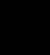
\includegraphics[width=.25in]{../presentation/2x2/Shape1LVL1.png}~
    
\includegraphics[width=.25in]{../presentation/2x2/Shape2LVL1.png} \\
\tiny{none} & 2 & empty \\
\tiny{($<$ x 1), ($<$ y 1), ($<$ x y), ($<$ 0 x), ($<$ 0 y), ($<$ y x)} & 3 & 
    
\includegraphics[width=.25in]{../presentation/2x2/Shape1LVL3.png}~
    
\includegraphics[width=.25in]{../presentation/2x2/Shape2LVL3.png}~
    
\includegraphics[width=.25in]{../presentation/2x2/Shape5LVL3.png}~
    
\includegraphics[width=.25in]{../presentation/2x2/Shape6LVL3.png}~
    
\includegraphics[width=.25in]{../presentation/2x2/Shape3LVL3.png}~
    
\includegraphics[width=.25in]{../presentation/2x2/Shape4LVL3.png}\\
\tiny{(not ($<$ x y)), (not ($<$ y x))} & 4 & 
    
\includegraphics[width=.25in]{../presentation/2x2/Shape2LVL4.png}~
    
\includegraphics[width=.25in]{../presentation/2x2/Shape1LVL4.png} \\
\tiny{($<$ (y + x) 1), ($<$ (y * x) 1), ($<$ 0 (y + x)), ($<$ 1 (y + x))} & 5 & 
    
\includegraphics[width=.25in]{../presentation/2x2/Shape2LVL5.png}~
    
\includegraphics[width=.25in]{../presentation/2x2/Shape1LVL5.png}~
    
\includegraphics[width=.25in]{../presentation/2x2/Shape3LVL5.png}~
    
\includegraphics[width=.25in]{../presentation/2x2/Shape4LVL5.png} \\
\tiny{none} & 6 & empty \\
\tiny{(or ($<$ y  x) ($<$ x  y))} & 7 &
    
\includegraphics[width=.25in]{../presentation/2x2/Shape1LVL7.png}\\
\tiny{(not (or ($<$ y  x) ($<$ x  y)))} & 8 &
    
\includegraphics[width=.25in]{../presentation/2x2/Shape1LVL8.png}
\end{tabular}
\end{center}

\caption{All the 2x2 art with its corresponding complexity.}
\label{fig:2x2}
\end{figure}

From Figure~\ref{fig:2x2}, some things are immediately obvious.  First of all,
as might match one's intuition, the all-black and all-white pictures are the
least complex pictures.  Secondly, one can see that if a formula of size $n$
exists to create a certain picture, then that picture's inverse has a
complexity of one of $n-1$, $n$, or $n+1$.  Examples of this last phenomenon
can be seen between rows 7 and 8, as well as between rows 3 and 4.  This occurs
for the simple reason that adding one symbol ({\tt not}) creates a picture's
inverse.  Also, somewhat intriguingly, we can see gaps at 2 and 6.  Although
there are formulae of size 2, none of those formulae produce a picture that has
not been already produced by formulae of a smaller size.

Seeing all of the pictures, our hypothesis becomes a bit more obvious: What is
the correlation between visual complexity (an inherently subjective notion) and
Kolmogorov complexity?  

